\documentclass{beamer}
\usepackage{amsfonts}
\usepackage{amsmath}
\usetheme{CambridgeUS}
\usecolortheme{seahorse}
\setbeamersize{text margin left=0.75cm,text margin right=0.75cm} 
\setbeamertemplate{navigation symbols}{}
\setbeamertemplate{itemize items}[default]
\setbeamertemplate{enumerate items}[default]
\setbeamertemplate{mini frames}{}
\setbeamercolor{alerted text}{fg =red}
\usepackage{framed}
\usepackage{tikz}
\usetikzlibrary{patterns}
\definecolor{blu}{RGB}{0, 64, 161}
\usepackage[]{textpos}
\usepackage{multirow}
\usepackage[makeroom]{cancel}
\usepackage{color}
\usepackage{colortbl}
\usepackage{libertine}
\usepackage{microtype}

\newcommand{\eps}{\varepsilon}
\newcommand{\vp}{\varphi}  %%
\newcommand{\bp}{\bar \varphi} %%
\newcommand{\bc}{\bar \chi} %%
\newcommand{\bV}{\bar V} %%
\newcommand{\bg}{\bar \gamma} %%
\newcommand{\al}{\alpha}
\newcommand{\hV}{\hat V} %%
%\newcommand{\Kh}{\hat K}
\newcommand{\hp}{\hat \phi} %%
\newcommand{\hk}{\hat k} %%
\newcommand{\hc}{\hat \chi} %%
\newcommand{\hatt}{\hat t} %%
\newcommand{\gmn}{g_{\mu\nu}}
\newcommand{\tgmn}{\tilde g_{\mu\nu}}
\newcommand{\bgmn}{\bar g_{\mu\nu}}
\newcommand{\hmn}{h_{\mu\nu}}
\newcommand{\thmn}{\tilde h_{\mu\nu}}
\newcommand{\hess}{\Gamma^{(2)}}
\newcommand{\eipx}{e^{i p\cdot x}}
\newcommand{\emipx}{e^{-ip \cdot x}}
\newcommand{\dclnf}{\,\partial_\chi\! \ln\! f \,}

\makeatletter
\def\maketag@@@#1{\hbox{\m@th\normalfont\footnotesize#1}}
\makeatother

\setbeamertemplate{footline}
{
  \leavevmode%
  \hbox{%
  \begin{beamercolorbox}[wd=.3\paperwidth,ht=2.25ex,dp=1ex,center]{author in head/foot}%
    \usebeamerfont{author in head/foot}\insertshortauthor
  \end{beamercolorbox}%
  \begin{beamercolorbox}[wd=.7\paperwidth,ht=2.25ex,dp=1ex,center]{title in head/foot}%
    \usebeamerfont{title in head/foot}\insertshorttitle\hspace*{3em}
    \insertframenumber{} / \inserttotalframenumber\hspace*{1ex}
  \end{beamercolorbox}}%
  \vskip0pt%
}

\newcommand{\eaa}{\hat\Gamma}
\newcommand{\bare}{\mathcal{S}}


\begin{document}

\title{Matter fields in the Asymptotic Safety scenario}
\author{Peter Labus}
\institute{SISSA Trieste
\vspace{5mm}
\\ \vspace{8pt}PL, T. R. Morris and Z. H. Slade, Phys. Rev. D 94 (2016)
\\ \vspace{8pt}P. Don\`a, A. Eichhorn, PL and R. Percacci, Phys. Rev. D93 (2016)
\\ \vspace{8pt}PL, R. Percacci, G.P. Vacca, Phys. Lett.  B753 (2016)
\\ \vspace{8pt}A. Eichhorn, PL, J. M. Pawlowski, M. Reichert, \textit{In preparation.}
\date{14/09/2017}
}
\begin{frame}[noframenumbering,plain]
	\titlepage
\end{frame}


%----------------------------------------------------------------------------------------
%   Section 1 --- Introduction
%----------------------------------------------------------------------------------------

\fontsize{8pt}{7.2}\selectfont

\section{Asymptotically safe quantum gravity}

\begin{frame}
  \frametitle{Why quantum gravity?}
  \textbf{Two pressing issues:}
  \begin{enumerate}
    \item singularities in GR (black holes, big bang)
      \hspace{2cm}
      \raisebox{-.5\height}{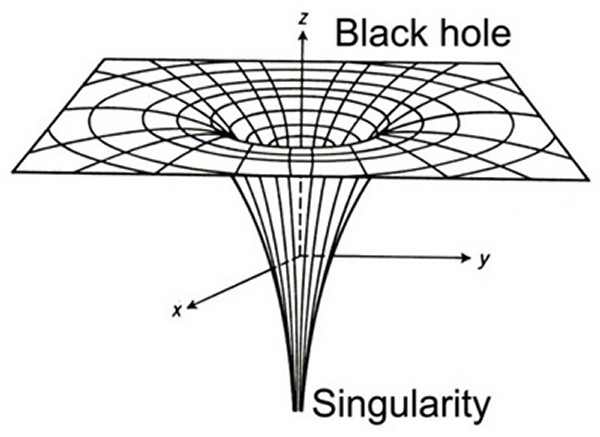
\includegraphics[width=0.25\textwidth]{blackholes_singularity.jpg}}
    \item singularities in SM (stability of electroweak sector)
      \hspace{1cm}
      \raisebox{-.5\height}{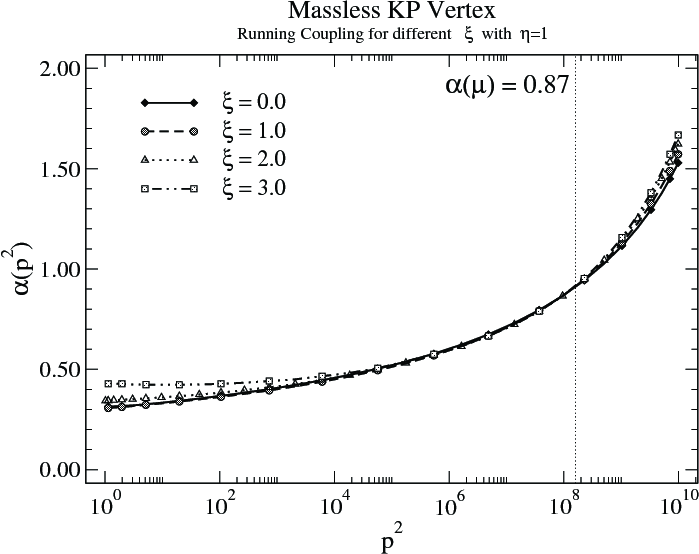
\includegraphics[width=0.25\textwidth]{running_alpha.png}}
  \end{enumerate}
  \vfill
  \pause
  \textbf{More theoretical issues:}\\[5pt]
  cosmological constant problem, hierarchy problem, origin of symmetries and field content,
  CP-violation, grand unification?, TOE?, \dots
\end{frame}

\begin{frame}
  \frametitle{Why quantum gravity?}
  \textbf{Two pressing issues:}
  \begin{enumerate}
    \item singularities in GR (black holes, big bang)
      \hspace{2cm}
      \raisebox{-.5\height}{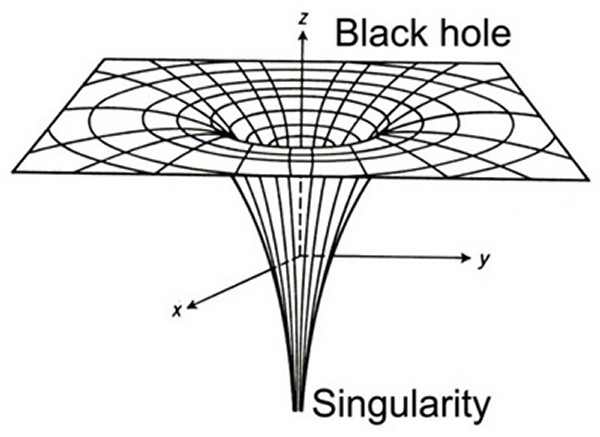
\includegraphics[width=0.25\textwidth]{blackholes_singularity.jpg}}
    \item singularities in SM (stability of electroweak sector)
      \hspace{1cm}
      \raisebox{-.5\height}{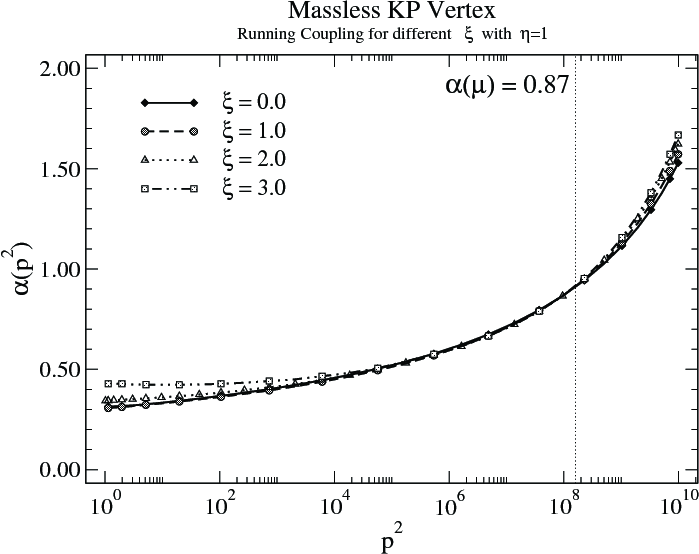
\includegraphics[width=0.25\textwidth]{running_alpha.png}}
  \end{enumerate}
  \vfill
  \begin{center}
    \fontsize{12pt}{7.2}\selectfont
    \textbf{ Can one help to cure the other? }
  \end{center}
  \pause
  \begin{center}
    candidates:\\[5pt]
    string theory, loop quantum gravity, causal dynamical triangulation, Regge calculus,\\
    causal sets, spin foams, group field theory, \dots
  \end{center}
\end{frame}

\begin{frame}
  \frametitle{Why quantum gravity?}
  \textbf{Two pressing issues:}
  \begin{enumerate}
    \item singularities in GR (black holes, big bang)
      \hspace{2cm}
      \raisebox{-.5\height}{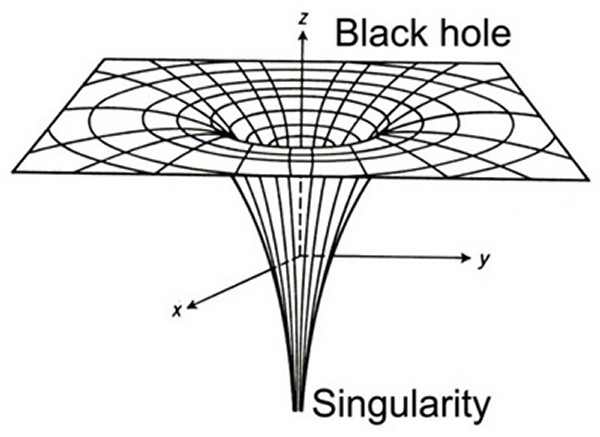
\includegraphics[width=0.25\textwidth]{blackholes_singularity.jpg}}
    \item singularities in SM (stability of electroweak sector)
      \hspace{1cm}
      \raisebox{-.5\height}{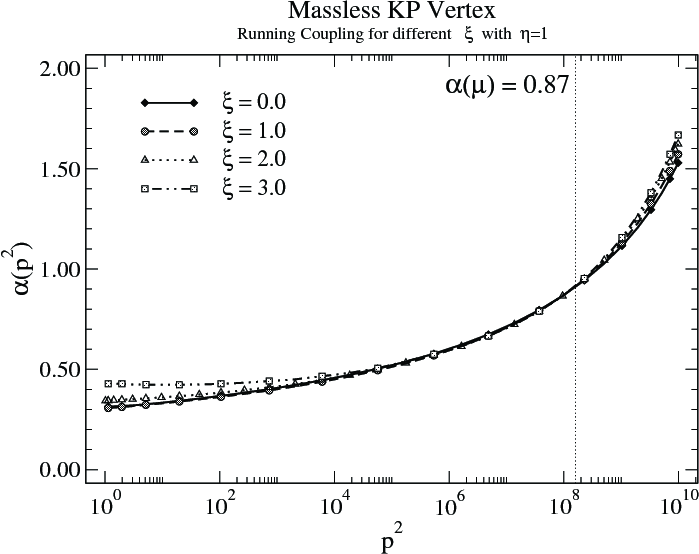
\includegraphics[width=0.25\textwidth]{running_alpha.png}}
  \end{enumerate}
  \vfill
  \begin{center}
    \fontsize{12pt}{7.2}\selectfont
    \textbf{ Can one help to cure the other? } \\[15pt]
    \textbf{ Have to go beyond QFTs? }
  \end{center}
\end{frame}

\section{Matter fields in asymptotic safety}
\section{Technical tools}
\section{Known issues}
\section{My research \& and its implications}


\end{document}
